\section{Evaluation}
\label{sec:evaluation}

To apply the policies and mechanisms discussed in section~\ref{sec:resilient-egde},
we implemented an image-processing application on Android platform, and its edge/cloud runtime services on Linux machines.
The edge device runtime is implemented as application-specfic runtime (section~\ref{sec:policy-fault}).
Thus we have the maximum flexibity to accommodate application-specifc requirement.

\subsection{Application}
\label{sec:eval-app}

The whole system consists three parts: mobile application, edge device runtime and cloud server runtime.

\hfill\break
\noindent \textbf{Mobile Application.}
We implemented an image-processing application on Android platform. The basic functionality is to classify
whether a user-supplied image contains a hotdog or not. The core hotdog classification program is an open-source
deep learning application~\cite{url:hotdog-classification} based on TensorFlow~\cite{tensorflow-osdi}.
We can only run the hotdog classification program on Linux servers, because it is developed before the
release of TensorFlow Lite~\cite{url:tensorflow-lite}, which is TensorFlow's lightweight soluton for mobile and embedded devices.
Therefore, we will not consider running computation on the local mobile device, computation is pushed to either
edge devices or cloud servers.
In case of edge device failure, we implemented the mechanisms described in section~\ref{sec:mechanism-fault}.

\hfill\break
\noindent \textbf{Cloud Server Runtime.}
Cloud server runtime is a multithread process running on Linux servers.
It has a daemon thread keep listening for requests from either mobile or edge devices.
Besides, it also has multiple worker threads that perform image classification.
The classification is done by calling into TensorFlow runtime. Worker threads
are sleeping when no jobs are available, they will be waken up by listening thread whenever jobs arrived.
Currently, we only implement the cloud server runtime on a single machine.

\hfill\break
\noindent \textbf{Edge Device Runtime.}
Edge device runtime resembles most of logic as in cloud server runtime.
Since it is application-specific runtime, we implemented the required logic to push computation
to peer edge devices or cloud servers. We used the algorithm described in section~\ref{sec:load-balancing}
to implement load balancing. To provide high availability and reliability, we implemented the necessary
mechanisms to take over jobs that were pushed to cloud in case of WAN network failure.

\subsection{Testing Environment}
We developed our mobile application on a Redmi 2 Pro smartphone, which has a Cortex-A53 processor, 2GB DRAM,
running with Android 4.4.4.
Our edge device is a MacBook Pro, with Intel Core i7 and 8GB DRAM. The cloud server has two Intel Xeon
E5-2620 processors, 128GB DRAM, running with CentOS 7.1 distribution and the 3.10 Linux kernel.

{
\begin{figure}[th]
\begin{center}
	\centerline{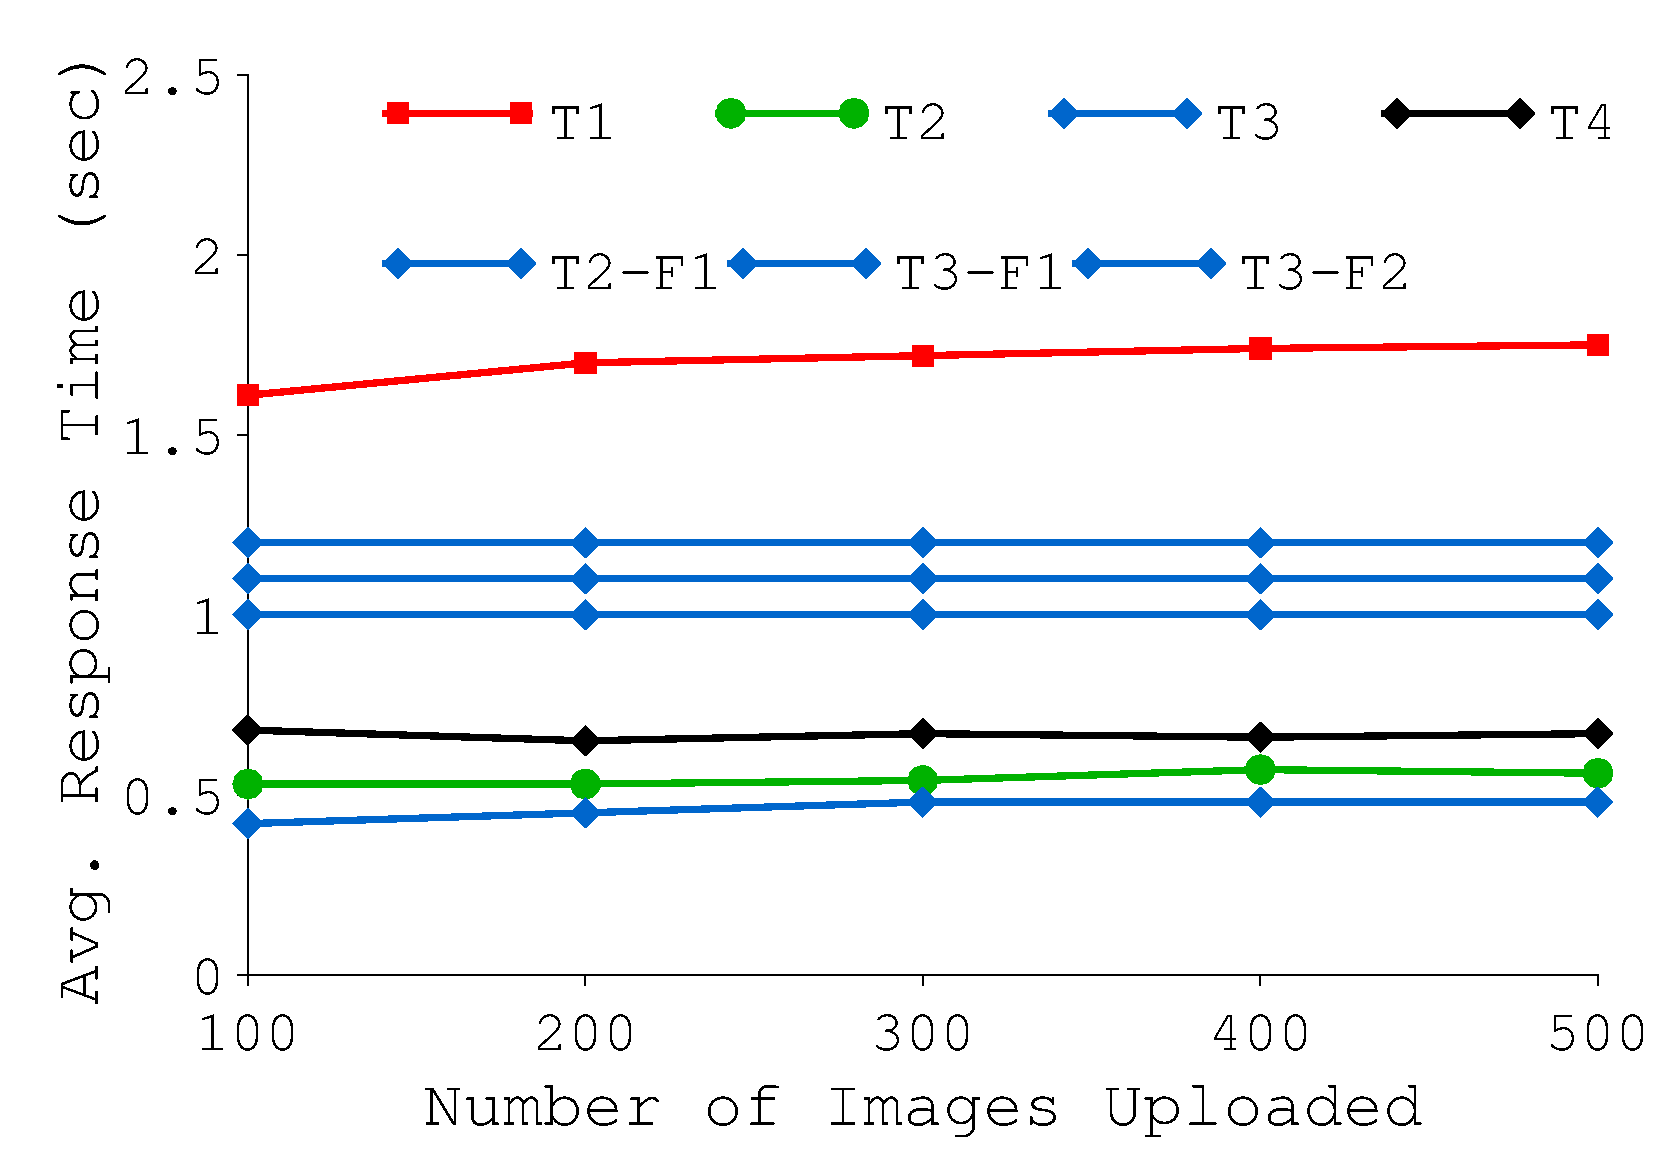
\includegraphics[width=2.5in]{Figures/g_plot_app.pdf}}
	\mycaption{fig-app}{Average Response Time Under Different Computing Models}
	{
	}
\end{center}
\end{figure}
}


\subsection{Result Analysis}
We experiment our system with all four computing models, as described in Figure~\ref{fig-computing-models}.
For type 1 and type 2, there is only one running edge device in the system. For type 3, we deploy two
edge devices. They are running in the same Macbook, but with different ports. In type 4, mobile device
send requests to cloud server directly, no edge device is deployed. Figure~\ref{fig-app} showed the
average response time of processing a user-supplied image. The response time including both network
delay and computation time.

Figure~\ref{fig-app} shows that type 4 has the best performance over others.
This contradicts our prediction simply because our Linux server has much stronger processing power
than our egde device (Macbook). The workload generated by our application is not able to saturate the server.
The strong processing power even offsets the gain of network. However, we consider in a real-world
environment cloud servers are normally highly utilized. The congestion of numerous concurrent
requests will saturate cloud servers, in which case the addition of edge servers will be able to
greatly improve the whole system throughtput.

asda
